\documentclass[12pt]{article}
% Chinese Support
\usepackage{xeCJK}
\setCJKmainfont{STSong}
% \setmainfont{Times New Roman}

% for symbol
\usepackage{gensymb}
% matrix
\usepackage{amsmath}

% For images
\usepackage{graphicx}
\graphicspath{ {./screenshoot/} }

\newcommand{\numpy}{{\tt numpy}}    % tt font for numpy

\topmargin -1.in
\textheight 9in
\oddsidemargin -.25in
\evensidemargin -.25in
\textwidth 7in


\usepackage{listings}
\usepackage{color}

\definecolor{dkgreen}{rgb}{0,0.6,0}
\definecolor{gray}{rgb}{0.5,0.5,0.5}
\definecolor{mauve}{rgb}{0.58,0,0.82}

\setmonofont{FiraCode-Regular}
\lstset{frame=tb,
  language=C++,
  aboveskip=3mm,
  belowskip=3mm,
  showstringspaces=false,
  columns=flexible,
  basicstyle={\small\ttfamily},
  numbers=none,
  numberstyle=\tiny\color{gray},
  keywordstyle=\color{blue},
  commentstyle=\color{dkgreen},
  stringstyle=\color{mauve},
  breaklines=true,
  breakatwhitespace=true,
  tabsize=3
}



% Content start below
\begin{document}

\author{陈铭涛\\ 16340024}
\title{计算机图形学 Homework 4 - Transformation}
\date{\vspace{-5ex}}
\maketitle

\medskip

% ========== Begin answering questions here

\section{Basics}

\begin{enumerate}

    \item \textbf{画一个立方体(cube):边长为4, 中心位置为(0, 0, 0)。分别启动和关闭深度测试,查看区别,并分析原因。}
    \begin{sloppypar}
        在 OpenGL 中画出立方体的方法为分别用两个三角形画出立方体的六个面。

        定义好6个面的36个顶点后使用\lstinline{ glDrawArrays(GL_TRIANGLES, 0, 36); }画出立方体。

        为了使立方体便于看出,对立方体以$y=2x$为轴进行了$45\degree$的旋转,变换矩阵为\lstinline{glm::rotate(model, glm::radians(45.0f), glm::vec3(0.5f, 1.0f, 0.0f));}.

        因为边长要求为4,所以需要另外向z轴方向调整摄像机位置以使得立方体可以完整显示在窗口内。方法为:
        \begin{lstlisting}
glm::lookAt( glm::vec3(0.0f, 0.0f, 10.0f),
             glm::vec3(0.0f, 0.0f, 0.0f),
             glm::vec3(0.0f, 1.0f, 0.0f));
        \end{lstlisting}

        最终显示的效果为:
        \begin{center}
            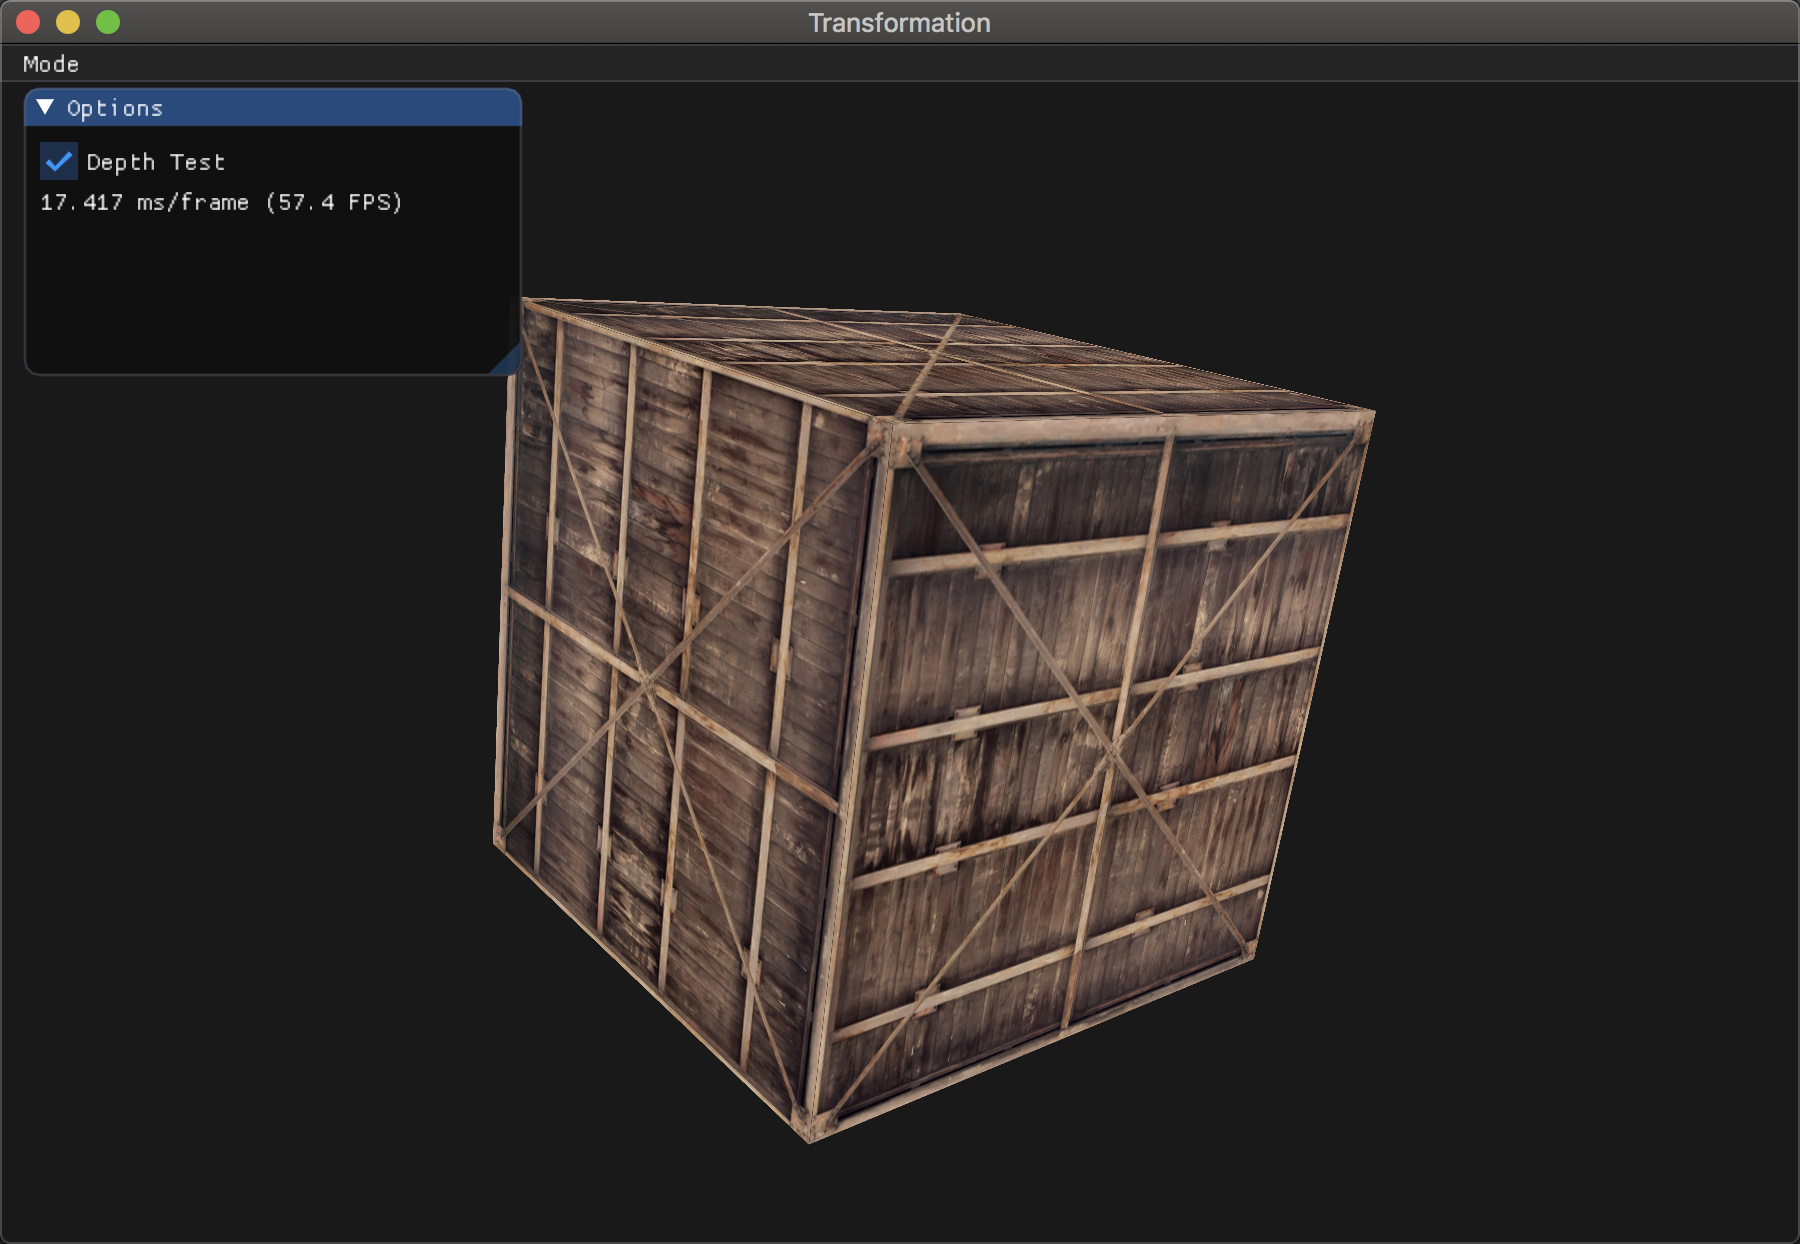
\includegraphics[scale=0.4]{static.png}
        \end{center}

        可通过 GUI 关闭深度测试,关闭深度测试的效果如下:
        \begin{center}
            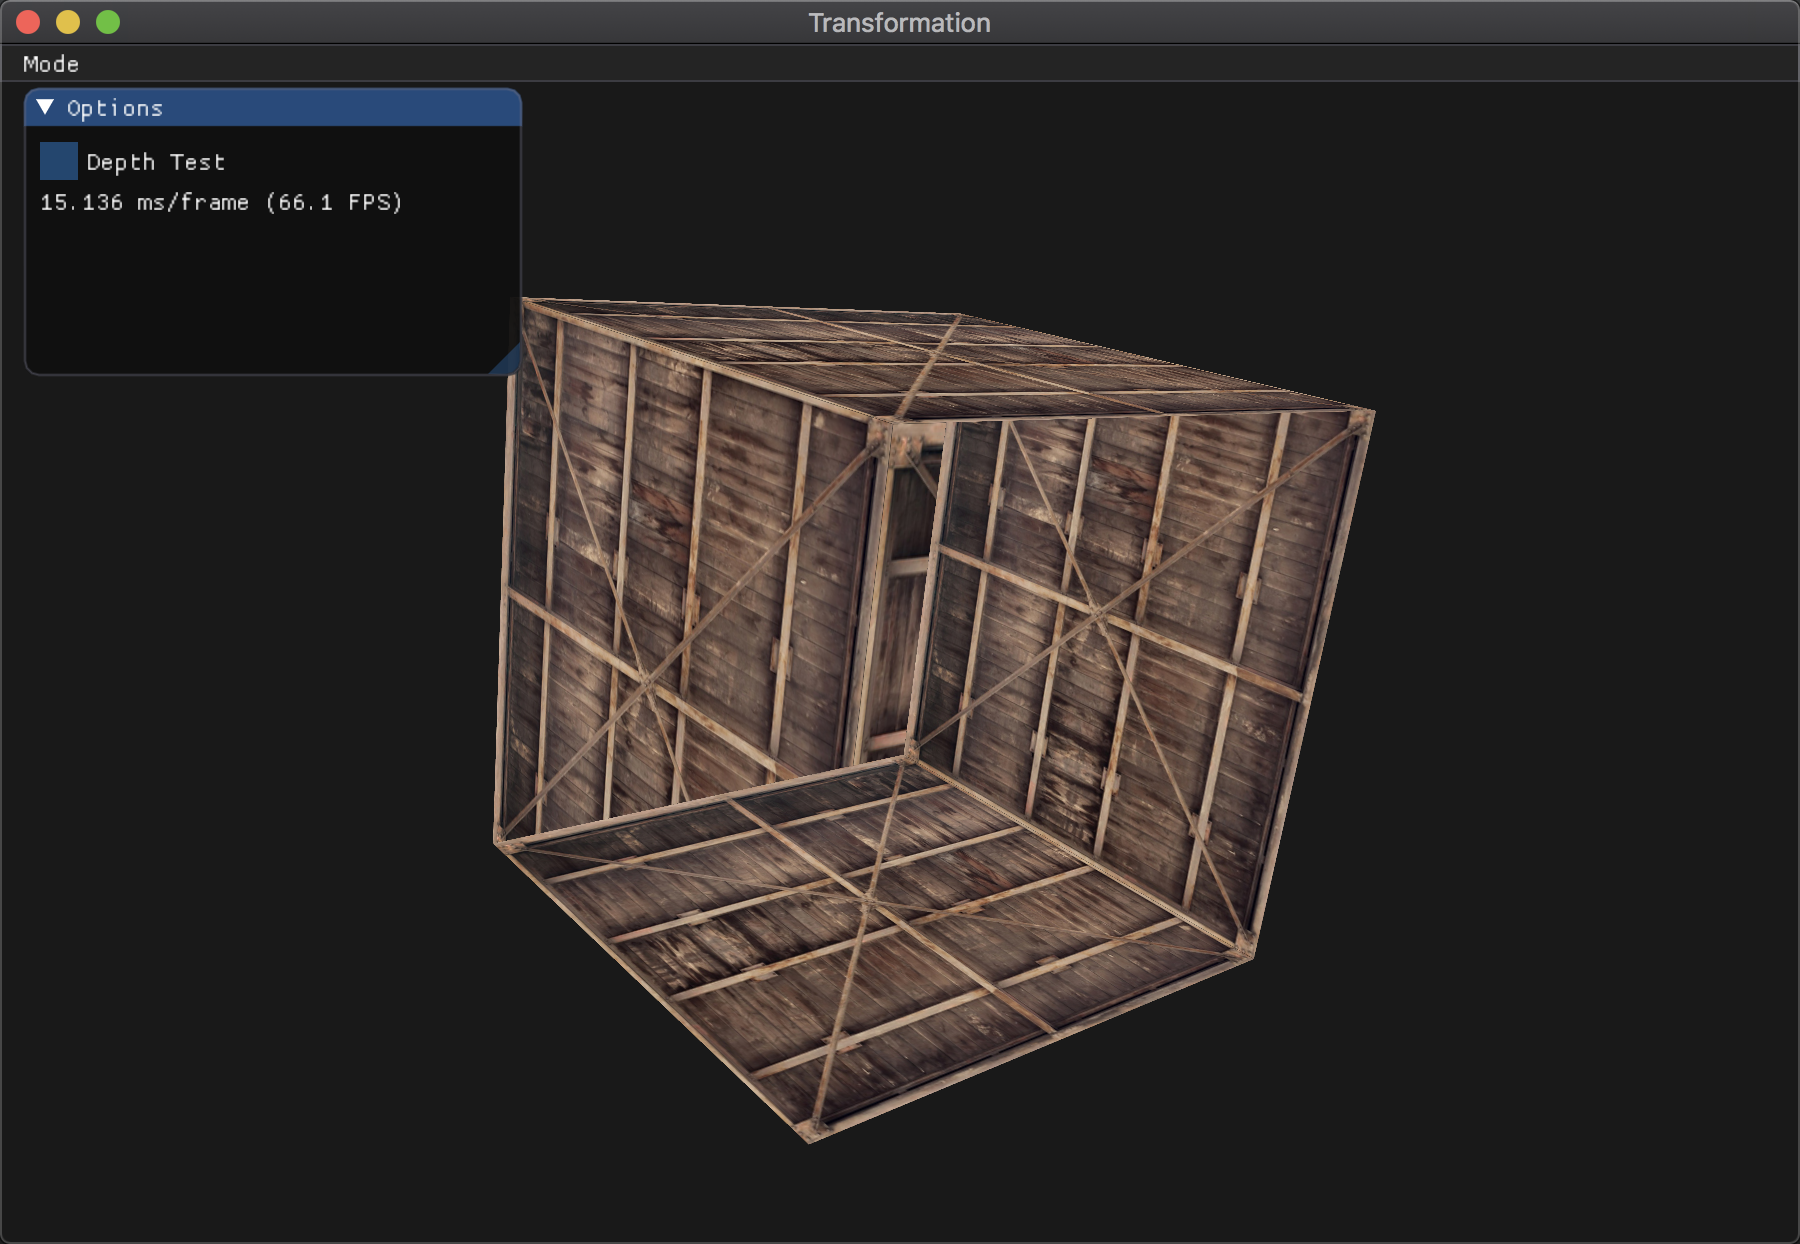
\includegraphics[scale=0.4]{NoDepthTest.png}
        \end{center}

        可看到关闭深度测试后本来应当被阻挡的面显示到了前方,影响了图形的真实感。

        需要开启深度测试的原因是开启后 OpenGL 将会把片段的深度值与深度缓冲的内容对比,若测试通过则深度缓冲的深度值成为新的深度值,若未通过则丢弃片段。通过这种方法可以清除场景中的不可见片段。每次绘制时需要清除深度缓冲区,即\lstinline{glClear(GL_DEPTH_BUFFER_BIT);}.
    \end{sloppypar}
    

    \item \textbf{平移(Translation):使画好的cube沿着水平或垂直方向来回移动。}
    
    位移的变换矩阵形如:
    \begin{equation}
    \begin{bmatrix}
        1 & 0 & 0 & -dx\\
        0 & 1 & 0 & -dy\\
        0 & 0 & 1 & -dz\\
        0 & 0 & 0 & 0
    \end{bmatrix}
    \end{equation}

    位移的方法为通过位移的变换矩阵进行,在 GLM 库中方法如下:
    \begin{lstlisting}
        if (horizontal) {
            x = sin((float)glfwGetTime()) * movingLength;
        }
        if (vertical) {
            y = cos(float(glfwGetTime())) * movingLength;
        }
        view = glm::translate(view, glm::vec3(x, y, 0));
    \end{lstlisting}
    立方体将根据时间进行水平或垂直方向的在一定范围内不断移动,当水平和垂直方向同时位移时,由于$x^2 + y^2 = l^2$, 立方体的运动轨迹将是半径为 movingLength 的圆。

    平移模式下的显示效果如下:
    \begin{center}
        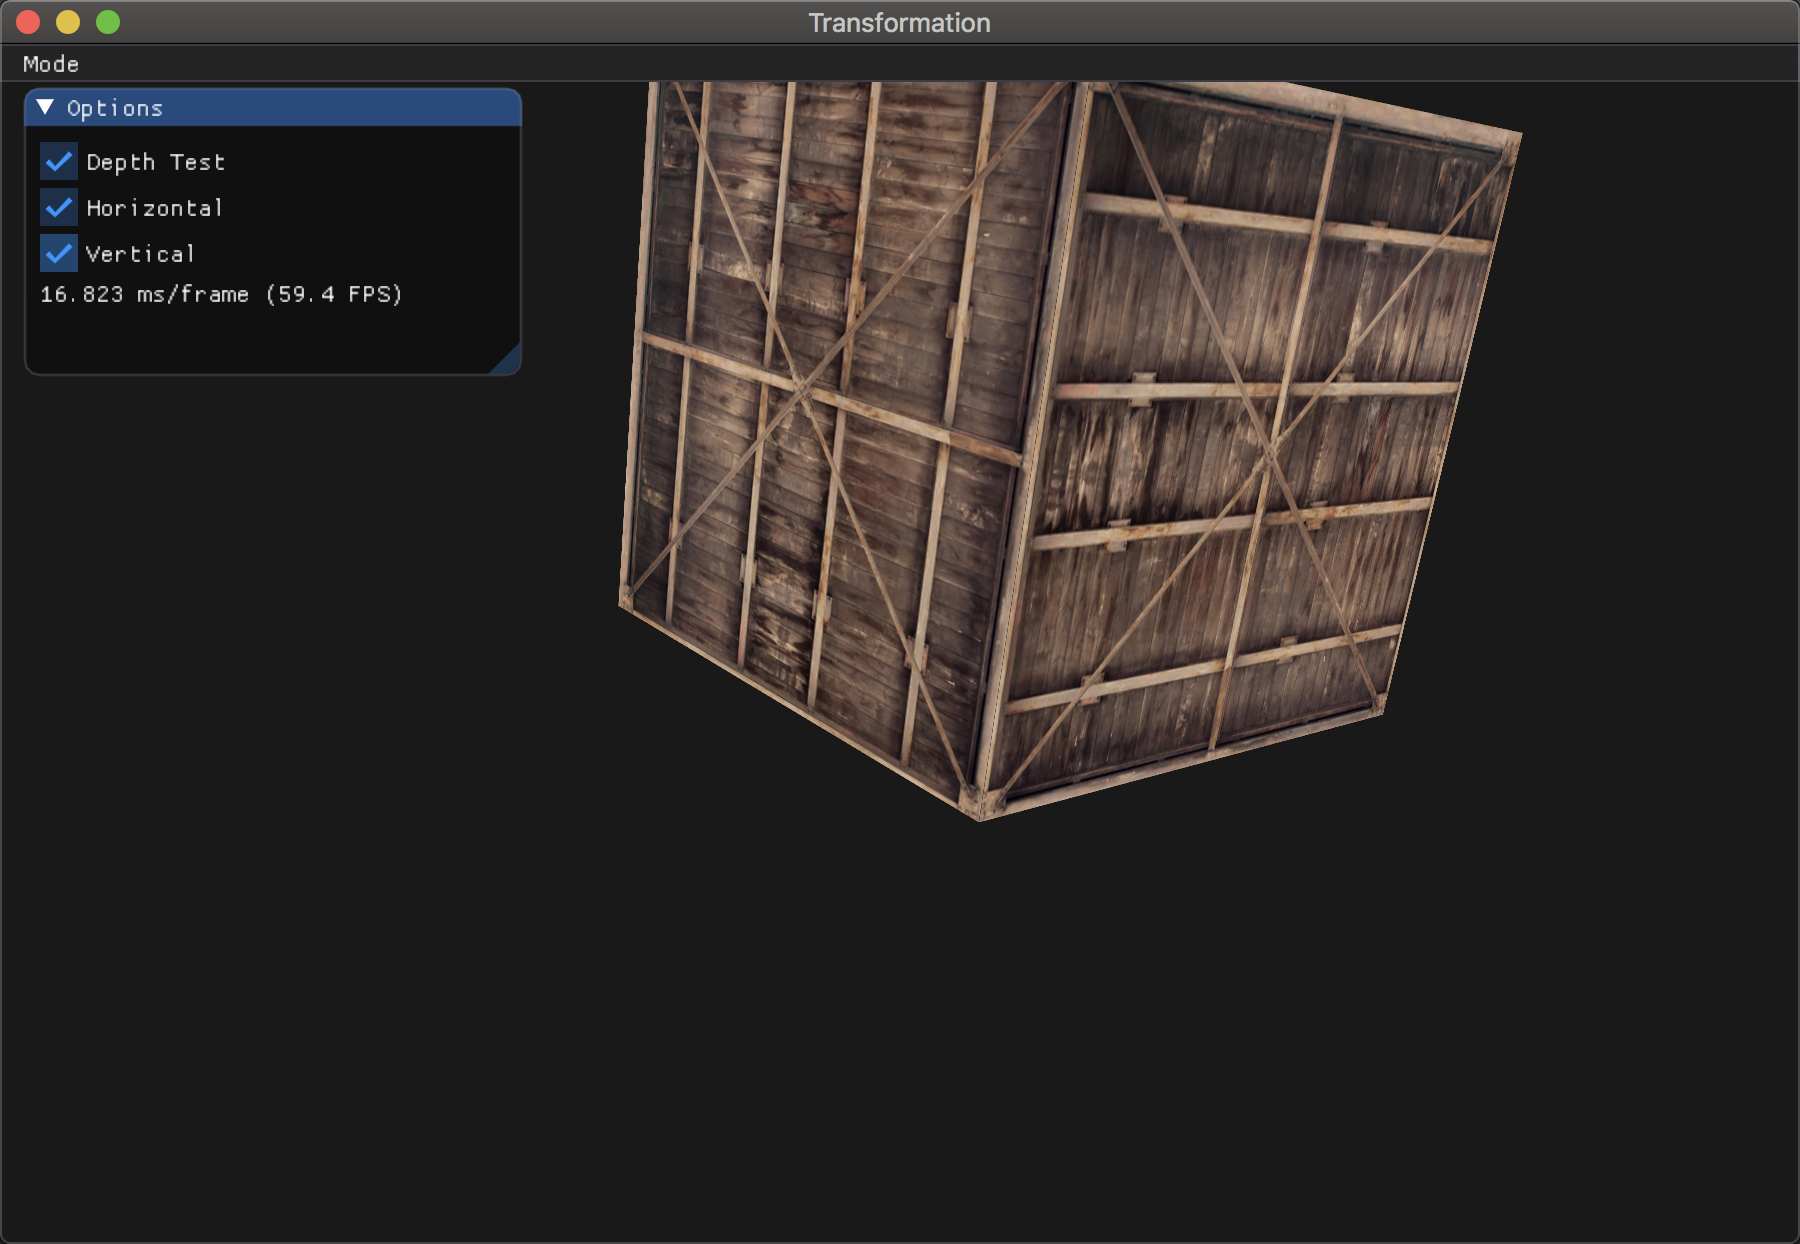
\includegraphics[scale=0.35]{translation.png}
    \end{center}

    \item 旋转(Rotation):使画好的cube沿着$XoZ$平面的$x=z$轴持续旋转。
    
    旋转的变换矩阵形如(延$x$轴):
    \begin{equation}
    \begin{bmatrix}
        1 & 0 & 0 & 0\\
        0 & cos\theta & sin\theta & 0\\
        0 & -sin\theta & cos\theta & 0\\
        0 & 0 & 0 & 0
    \end{bmatrix}
    \end{equation}

    根据时间计算旋转角度,计算变换矩阵后达成效果,每旋转一周期时间为3.6秒:
    \begin{lstlisting}
        auto weight = static_cast<float>(fmod(float(glfwGetTime()), 3.6));
        model = glm::rotate(model, glm::radians(weight * 100.0f), axis);
    \end{lstlisting}

    旋转效果如下:
    \begin{center}
        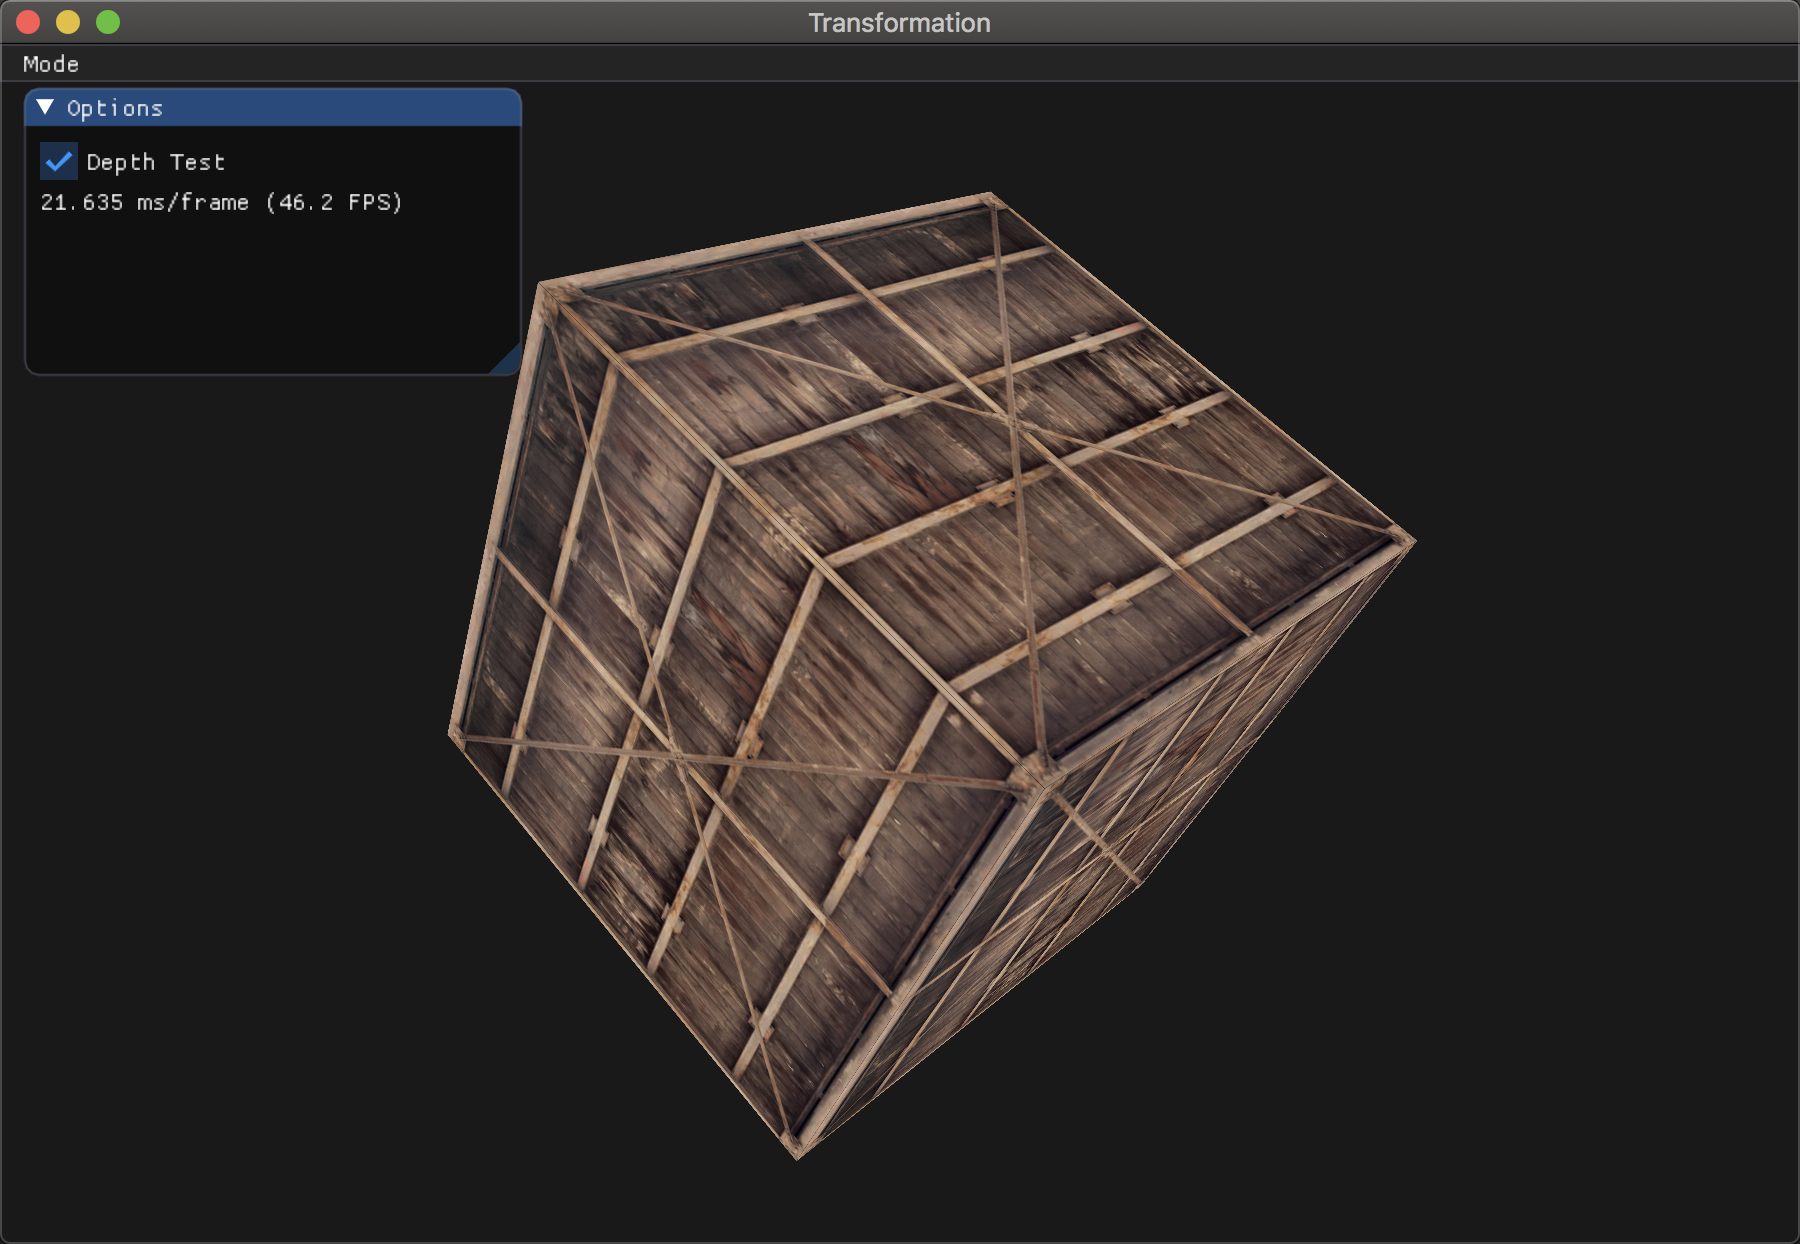
\includegraphics[scale=0.35]{rotating.png}
    \end{center}

    \item 放缩(Scaling):使画好的cube持续放大缩小。
    
    缩放的变换矩阵形如(延$x$轴):
    \begin{equation}
    \begin{bmatrix}
        S_x & 0 & 0 & 0\\
        0 & S_y & 0 & 0\\
        0 & 0 & S_z & 0\\ 
        0 & 0 & 0 & 0
    \end{bmatrix}
    \end{equation}

    根据时间计算缩放的大小,进行缩放的方法是在先前变换的基础上乘入缩放变换矩阵,使用 GLM 库中方法如下:
    \begin{lstlisting}
        auto factor = static_cast<float>((sin(glfwGetTime()) + 1) * 0.9 + 0.2);
        model = glm::scale(model, glm::vec3(factor, factor, factor));
    \end{lstlisting}
    缩放的效果如下:
    \begin{center}
        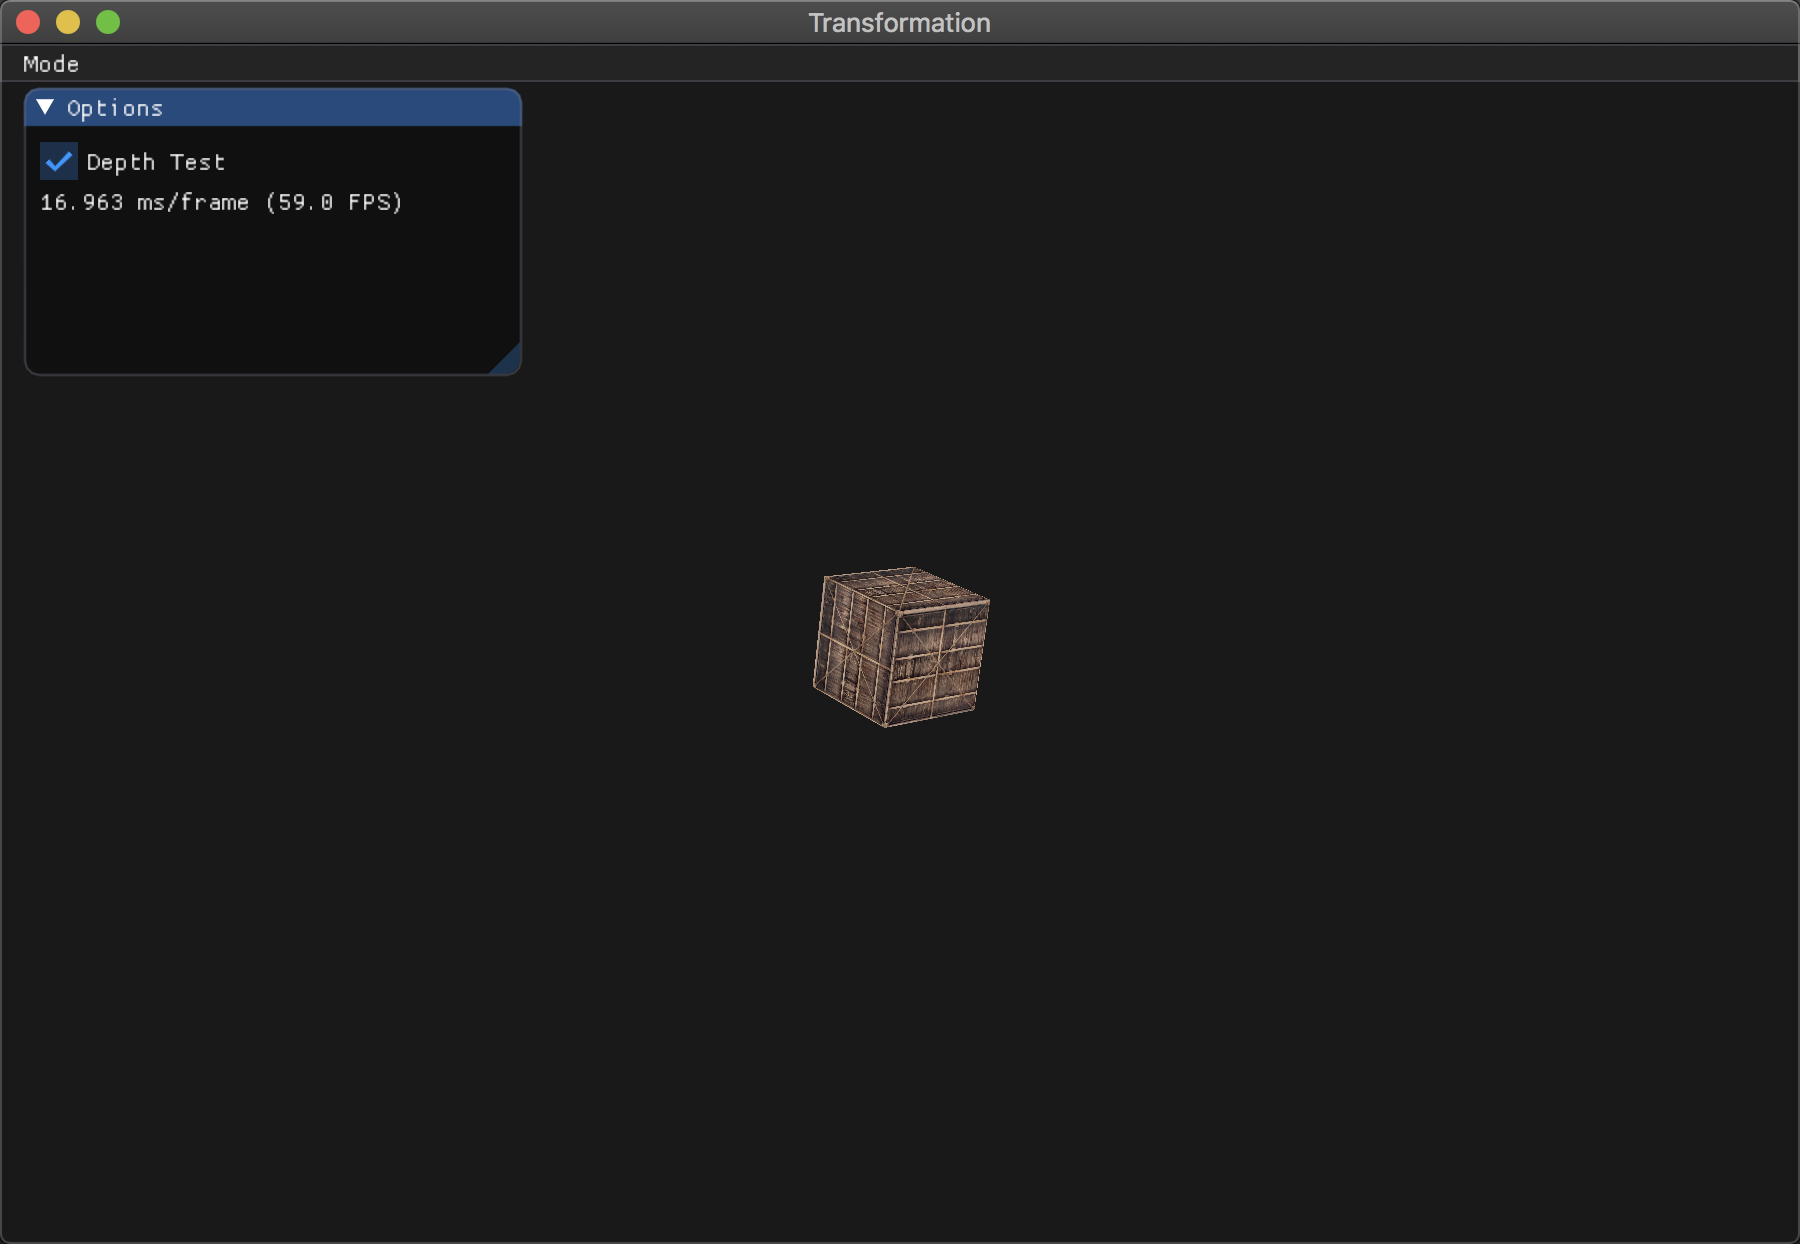
\includegraphics[scale=0.4]{scaling.png}
    \end{center}

    \item 在GUI里添加菜单栏,可以选择各种变换。

    菜单栏效果如下:
    \begin{center}
        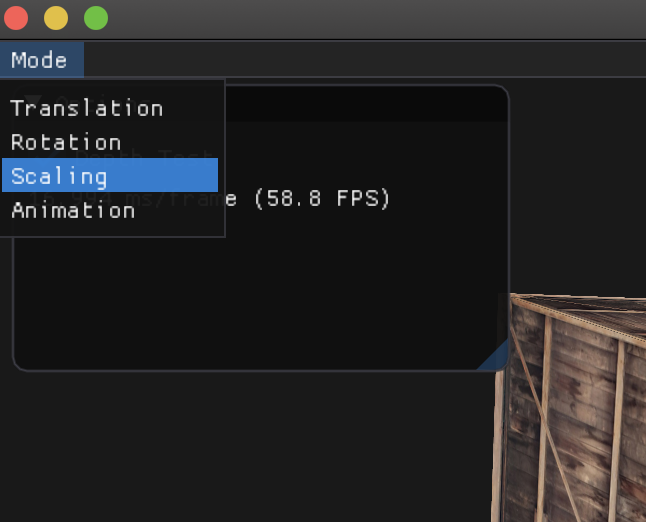
\includegraphics[scale=1]{GUI.png}
    \end{center}

    \item 结合Shader谈谈对渲染管线的理解
    
    渲染管线包含顶点处理(对应顶点着色器),几何处理(几何着色器),裁剪阶段及光栅化阶段(对应片段着色器)。
    
    在固定管线中,图形的绘制渲染被封装为API,通过 API 来配置管线的运行,抽象了许多细节,操作的局限性较大,虽易于理解,但是灵活性与效率都不高。

    在可编程管线中,图形渲染主要通过对着色器的实现,有更高的自由度,通过着色器的编程来实现图像的效果。如顶点着色器可处理空间坐标变化、纹理变化等,片段着色器可处理片段颜色与纹理等效果。
    
    本次变换的实现依赖于顶点着色器,通过传入的变换矩阵实现从局部坐标系到世界坐标系,摄影坐标系,投影坐标系的变换。

    在本次作业的着色器中,接收了一个uniform 变换矩阵,并将变换矩阵与局部坐标相乘后获得变换后的顶点坐标:
    着色器:
    \begin{lstlisting}
        #version 330 core
        layout (location = 0) in vec3 pos;
        layout (location = 1) in vec2 textureCoord;
        out vec3 verColor;
        out vec2 texCoord;
        uniform mat4 transform;

        void main()
        {
            gl_Position = transform * vec4(pos, 1.0);
            verColor = vec3(1.0, 1.0, 1.0);
            texCoord = vec2(textureCoord.x, textureCoord.y);
        }
    \end{lstlisting}        
    传递:
    \begin{lstlisting}
    int transformLoc = glGetUniformLocation(shader->getProgram(), "transform");
    glUniformMatrix4fv(transformLoc, 1, GL_FALSE, glm::value_ptr(transformer->getTransformMatrix()));
    \end{lstlisting}

\end{enumerate}


\section{Bonus}
    \emph{将以上三种变换相结合,打开你们的脑洞,实现有创意的动画.}
    \\[20pt]
    \indent 实现的内容为地球围绕太阳的公转运动与自转,使用不同纹理的立方体来表示太阳与地球。

    设置的太阳与地球的自转速度为3.6秒每周期,旋转轴分别为$y$轴与$z$轴。

    地球公转为一个椭圆形,椭圆的标准方程为
    \begin{equation}
        \frac{x^2}{a^2} + \frac{y^2}{b^2}=1
    \end{equation}

    在实现中(位于 Transformation.cpp下的EllipseTransform类)的公式为:
    \begin{equation}
        \begin{aligned}
            x = a\cos t\\
            y = b\sin t
        \end{aligned}
    \end{equation}

    太阳的坐标位于(-b, 0, 0), 由于地球公转在近日点和远日点的速度不同,此处的实现方法是令位移速度随地球所在的 x 坐标越接近-a而越小,使得地球接近太阳时位移加快,远离太阳时位移减慢。该效果可通过取消 GUI 中 Dynamic Speed 选项来关闭。

    动画效果如下:
    \begin{center}
        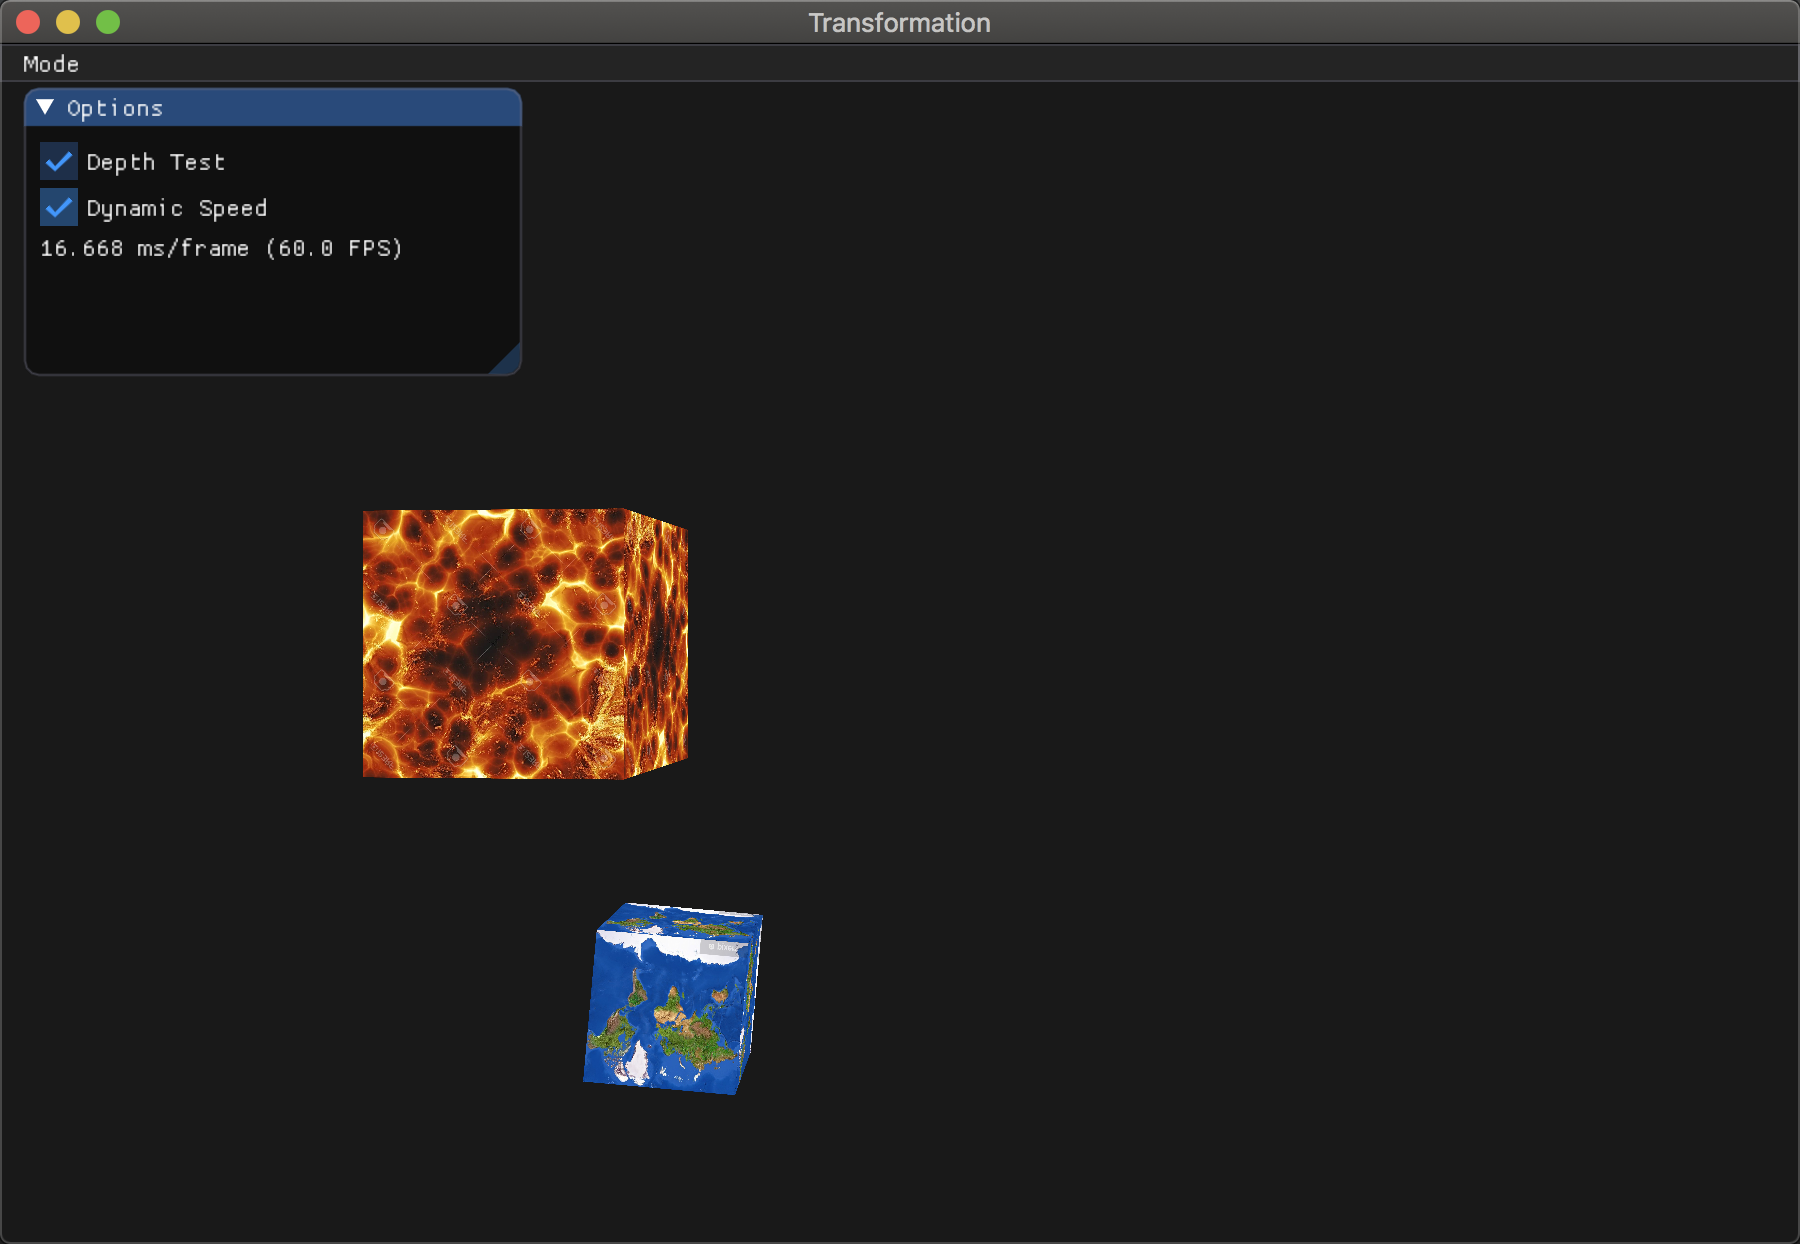
\includegraphics[scale=0.4]{orbit.png}
    \end{center}

\end{document}
\grid
\grid